\part{Part 3:}

\chapter{Quantum Neuromorphic Computing}
\section{System Dynamics-Based Methods}\index{System Dynamics-Based Methods}
\section{Neuron Simulation Methods}\index{Neuron Simulation Methods}



% \part{Parte Dos}

% % ----------------------------------------------------------------------------------------
% %	  CHAPTER 3
% % ----------------------------------------------------------------------------------------

% \chapterimage{ima2} % Chapter heading image


% %Anexos
% \chapter*{Anexos}
% \addcontentsline{toc}{chapter}{\textcolor{ocre}{Anexos}}

% Anexo1: Representación gráfica de la función logística
% \begin{center}
% 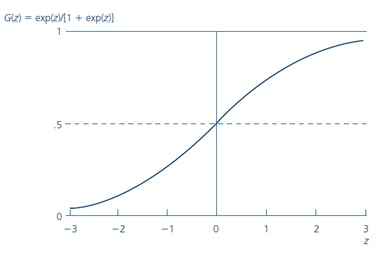
\includegraphics[height=5.5cm]{ima11}
% \end{center}

% Anexo2: Resultados de la aplicación del Modelo Probit
% \begin{center}
% 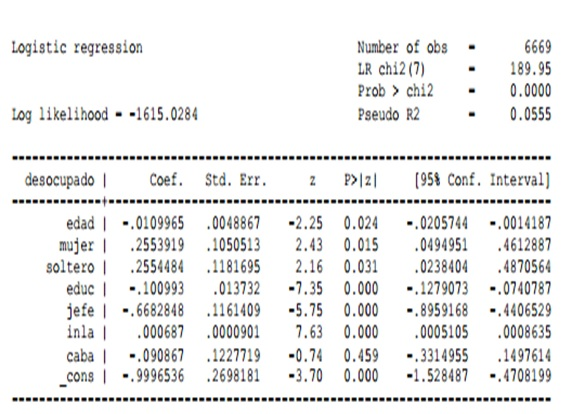
\includegraphics[height=6.5cm]{kat1}
% \end{center}

% Anexo3: Resultados de la estimación con el Modelo Logit
% \begin{center}
% 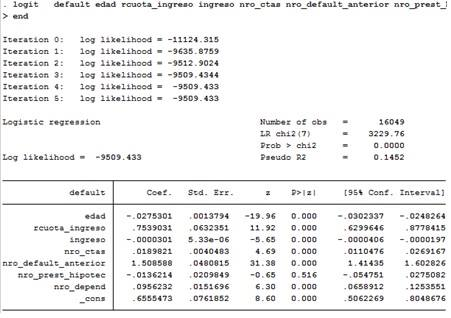
\includegraphics[height=8.5cm]{picture11}
% \end{center}

% Anexo4: Resultados del Test de Wald
% \begin{center}
% 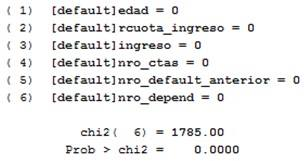
\includegraphics[height=4cm]{picture8}
% \end{center}

% Anexo5: Resultados de la segunda estimación con el Modelo Logit \begin{center}
% 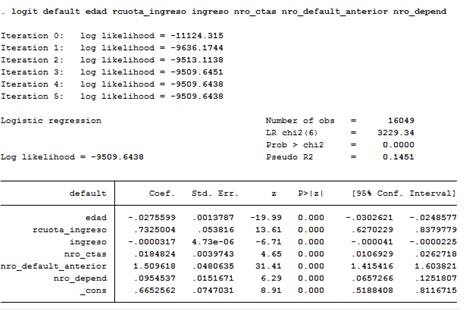
\includegraphics[height=8.5cm]{picture7}
% \end{center}

% \newpage
% Anexo6: Resultados de la estimación con el Modelo Probit
% \begin{center}
% 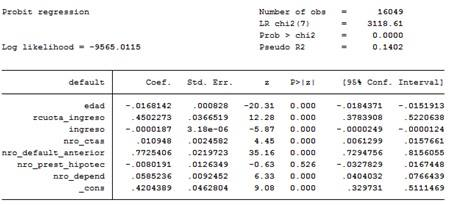
\includegraphics[height=6.5cm]{picture1}
% \end{center}

% Anexo7: Resultados de la segunda estimación con el Modelo Probit
% \begin{center}
% 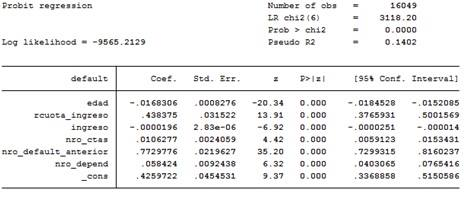
\includegraphics[height=6.5cm]{picture10}
% \end{center}

% Anexo8: Potencia de la predicción con el Modelo Logit
% \begin{center}
% 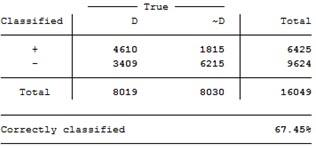
\includegraphics[height=5.5cm]{picture4}
% \end{center}

% \newpage
% Anexo9: Potencia de la predicción con el Modelo Probit
% \begin{center}
% 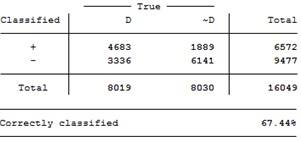
\includegraphics[height=5.5cm]{picture3}
% \end{center}

% Anexo10: Representación gráfica de la Curva ROC
% \begin{center}
% 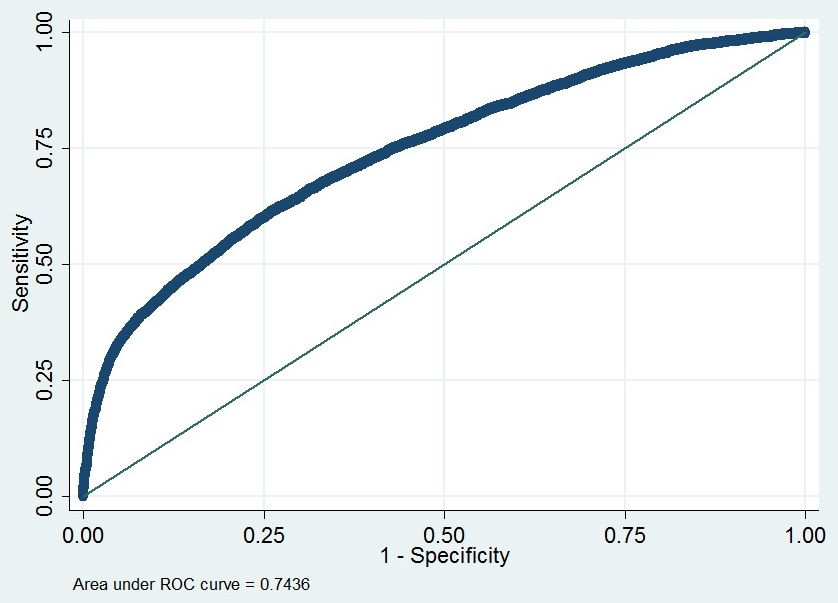
\includegraphics[height=7cm]{picture16}
% \end{center}

% Anexo11: Valor esperado de la PD por categoría
% \begin{center}
% 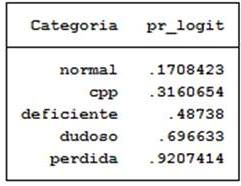
\includegraphics[height=5.5cm]{picture6}
% \end{center}

% Anexo12: Pérdida esperada de la entidad financiera ABC por categoría
% \begin{center}
% 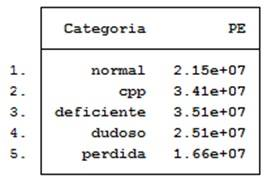
\includegraphics[height=5.5cm]{picture2}
% \end{center}


% %----------------

% %----------------------------------------------------------------------------------------
% %	BIBLIOGRAPHY
% %----------------------------------------------------------------------------------------

% \chapter*{Bibliografía}
% \addcontentsline{toc}{chapter}{\textcolor{ocre}{Bibliografía}}
% \section*{Books}
% \addcontentsline{toc}{section}{Books}
% \printbibliography[heading=bibempty,type=book]

% \begin{itemize}
% 	\item GREENE, W.H. (2003) “Econometric Analysis”5ª edición. Prentice Hall N.J. Capítulo 21
% \\\\
%     \item WOOLDRIDGE, J.M. (2010) “Introducción a la Econometría: Un Enfoque Moderno". 4ª edición. Cengage Learning. Capítulo 17

% \end{itemize}
